\section*{Problemas PID: }
    Considerando-se o sistema:  
    \begin{equation*}
        G = \frac{0.25(K_d s^2 + K_p s +K_i)}{s(s+1)(s+5)}
    \end{equation*}
    
    Em que $K_d = 150.88$, $K_p = 1373.92$ e $K_i = 5000$
    
    \subsection*{a) Utilize o MATLAB e realize as simulações do sistema em malha 
    fechada no domínio do tempo contínuo.}

        Primeiro, foram definidas as funções de transferência (FT) da planta, do controlador e então obteve-se 
        o ganho em malha aberta (MA) e em malha fechada (MF), posto que esse conjunto de FT serão utilizados por várias
        questões. O bloco de código \ref{DefFT} apresenta

        \begin{lstlisting}[language=Matlab,label=DefFT,caption=Definindo FTs]
            %Planta
            Nump = 0.25;
            Denp = conv([1 1], [1 5]);
            H = tf(Nump, Denp);
            
            %Controlador
            Kp = 1373.92;
            Ki = 5e3;
            Kd = 150.88;
            
            Numc = [Kd Kp Ki];
            Denc = [1 0];
            Gc =  tf(Numc, Denc);
            
            %Ganho em Malha Aberta
            Gma = H*Gc;
            
            %Ganho em Malha Fechada
            Gmf = Gma/(1+Gma);
        \end{lstlisting}

        Para observar o comportamento do sistema em MF, utilizou-se da entrada a degrau, como mostrado 
        no bloco de código \ref{DQ1}. 

        \begin{lstlisting}[language=Matlab,label=DQ1,caption=Resposta ao degrau]
            %% Q a)
            [y,t] = step(Gmf, 0.35);
            figure
            plot(t, y, 'LineWidth', 2);
            legend('c(t)')
            grid        
        \end{lstlisting}

        Ao utilizar \mcode{[y,t] = step(Gmf)} a função \mcode{step} não gera um gráfico
        mas sim, retorna vetores ``\mcode{y}'' e ``\mcode{t}'' referentes às posição dos pontos. Essa abordagem foi utilizada  
        nesse e nos próximos códigos com a finalidade de realizar ajustes no gráfico como o de adicionar legenda e o de aumentar 
        a espessura da curva. O resultado obtido pode ser visto na Figura \ref{fig1a}.

        \begin{figure}[!h]
            \centering
            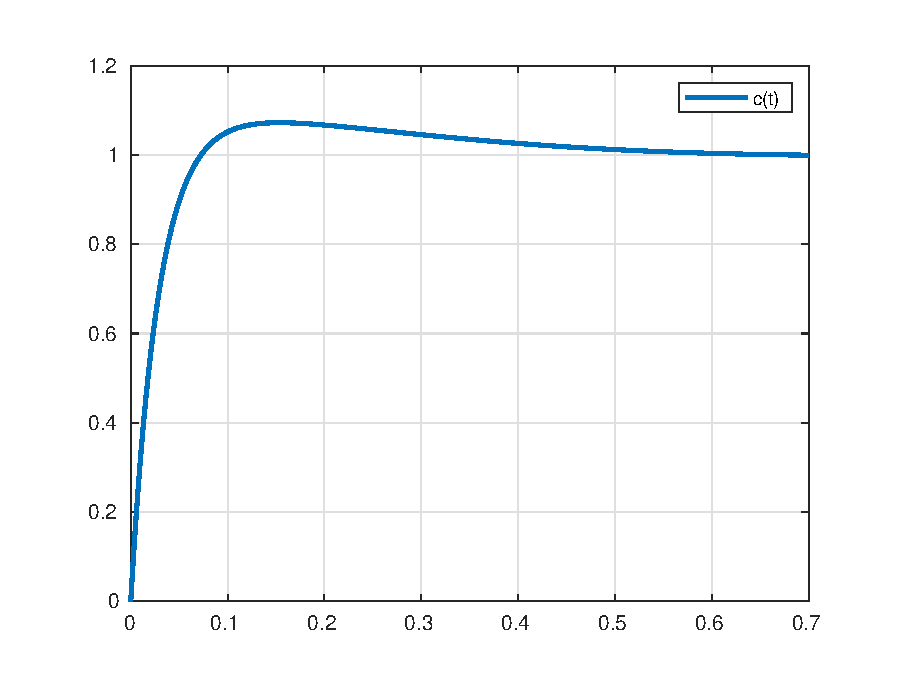
\includegraphics[width = 0.75\linewidth]{Figuras/ProblemaPID/step.eps}
            \caption{Gráfico da resposta ao degrau do sistema}
            \label{fig1a}        
        \end{figure}

    \subsection*{b) Determine o LGR  sem e com controlador}
        O lugar geométrico das raízes (LGR) pode ser facilmente obtido através da função \mcode{rlocus} nativa do matlab. 
        O sistema sem o controlador é constituido unicamente da planta do sistema. O LGR do sistema com o controlador, por outro 
        lado, é o produto no domínio ``s'', da FT do controlador com a FT da planta. O gráfico \ref{} apresenta os respectivos 
        LGRS 
        
        \begin{figure}[!h]
            \centering
            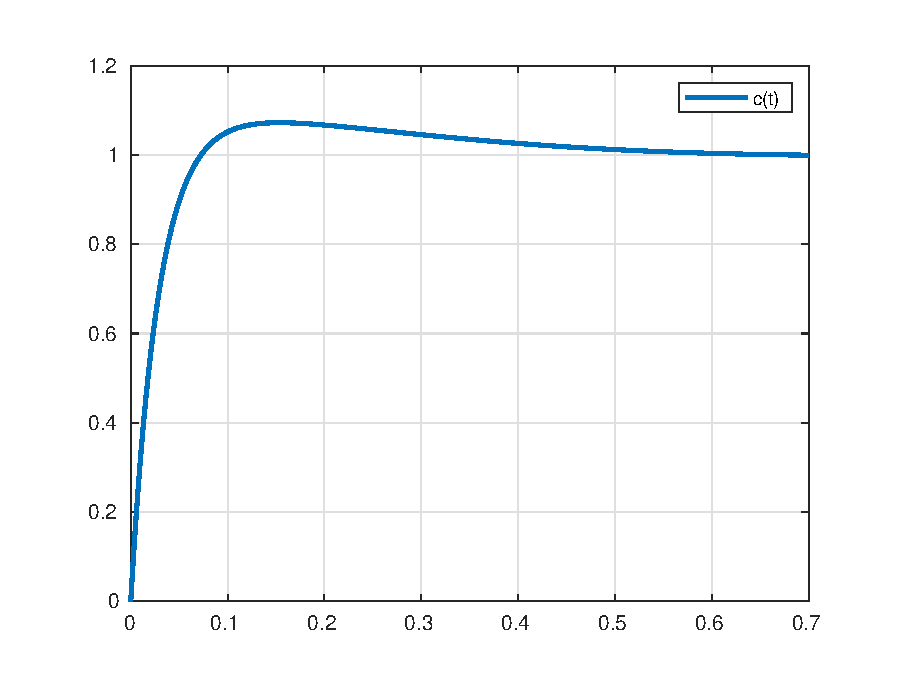
\includegraphics[width = 0.75\linewidth]{Figuras/ProblemaPID/step.eps}
            \caption{Gráfico da resposta ao degrau do sistema}
            \label{fig1a}        
        \end{figure}